\documentclass[12pt]{extarticle}
\usepackage{amsmath, amsthm, latexsym, tikz, graphicx, listings, microtype, mathtools, soul, color, fancyhdr, pgfplots, filecontents}
\usepackage[margin=1in]{geometry}
\pgfplotsset{width=15cm,height=10cm,compat=1.13}

%Timing data gathered on Joshua Higginbotham's MacBook Pro,
%used to make the example graph
\begin{filecontents*}{testdata.csv}
w,usecs
20,6227032
25,4984267
30,4154714
35,3587760
40,3146142
45,2822256
50,2550766
55,2303931
60,2115760
65,1958458
70,1821863
75,1705560
80,1598997
85,1511727
90,1427361
95,1356797
100,1284811
105,1228262
110,1169654
115,1121278
120,1081317
125,1040008
130,1006671
135,962837
140,925167
145,895679
150,871183
155,847787
160,832181
165,792484
170,768953
175,744501
180,726273
185,708575
190,692679
195,678567
200,706424
205,661261
210,651291
215,623957
220,608975
225,597934
230,609772
235,578803
240,606318
245,581887
250,547820
300,538680
400,594374
500,700618
600,748922
700,787258
800,726860
900,903822
1000,821859
1100,839192
1200,886371
1300,898255
1400,958942
1500,1077546
1600,1020523
1700,1060130
1800,1049812
1900,19229150
\end{filecontents*}

\newenvironment{myindentpar}[1]%
 {\begin{list}{}%
         {\setlength{\leftmargin}{#1}}%
         \item[]%
 }
 {\end{list}}
 
\DeclarePairedDelimiter\abs{\lvert}{\rvert}%
\DeclarePairedDelimiter\norm{\lVert}{\rVert}%

% Swap the definition of \abs* and \norm*, so that \abs
% and \norm resizes the size of the brackets, and the 
% starred version does not.
\makeatletter
\let\oldabs\abs
\def\abs{\@ifstar{\oldabs}{\oldabs*}}
%
\let\oldnorm\norm
\def\norm{\@ifstar{\oldnorm}{\oldnorm*}}
\makeatother

\definecolor{lightgray}{gray}{0.65}
\definecolor{pinegreen}{RGB}{1, 171, 161}
\definecolor{lightblue}{RGB}{135, 206, 250}
\definecolor{dkgreen}{rgb}{0,0.6,0}
\definecolor{gray}{rgb}{0.5,0.5,0.5}
\definecolor{mauve}{rgb}{0.58,0,0.82}
\definecolor{darkblue}{rgb}{0.0,0.0,0.6}
\definecolor{cyan}{rgb}{0.0,0.6,0.6}

\newcommand*{\Value}{\frac{1}{2}x^2}%
\newcommand{\hlc}[2][yellow]{ {\sethlcolor{#1} \hl{#2}} }


% /*--------------------------------------------------------------*/
%   Changing the values here sets the due date for the assignment!
% /*--------------------------------------------------------------*/
\newcommand{\duedate}{XX/XX/XX }
\newcommand{\semester}{SEMESTER}

\lstset{frame=tb,
  language=C++,
  breaklines=true,
  showstringspaces=false,
  columns=flexible,
  numbers=none,
  tabsize=3,
  escapeinside={(*@}{@*)}
  %,
  %commentstyle=\color{dkgreen},
  %stringstyle=\color{mauve}
}
\pagestyle{fancy}
\fancyhf{}
\renewcommand{\headrulewidth}{0pt}
\lhead{\color{lightgray} CSCE-313}
\rhead{\color{lightgray} \semester}
\rfoot{\thepage}
\pagenumbering{arabic}

\definecolor{codegray}{gray}{0.9}
\newcommand{\code}[1]{\colorbox{codegray}{\texttt{#1}}}

\begin{document}
\begin{center}
    \underline{{\large Machine Problem 7: UNIX Threads \  }(Due: \duedate)}  \\
\end{center}

\ \\
{\large \underline{Introduction}:}

\begin{myindentpar}{5mm}

    \noindent
    For many computing tasks it is sufficient that one instruction be executed immediately after another, sequentially, until the program completes. However, in the case that many tasks need to be executed at once, or that a single task can be appropriately split into sub-tasks, a program’s performance can be greatly improved by working on tasks concurrently or in parallel through the use of threads. Sometimes it works just as well to use multiple processes, or multitasking, instead of multithreading, but there are many benefits that result from multithreading.  

\end{myindentpar}

\ \\
{\large \underline{Threading Background}:}

\begin{myindentpar}{5mm}

    \noindent
    \textbf{How do threads differ from processes?}
    
    \vspace{-3mm}
    \ \\
    A process is a container for code in execution.  It consists of an address space which houses program code and all program data (See Advanced Concepts section for further information).  In UNIX/Linux operating systems, processes are maintained as completely separate execution units.  Any given process knows absolutely nothing about other processes executing on the system, and processes can only communicate using one of the IPC (Inter-Process Communication) mechanisms offered by the kernel (Named/unnamed pipes, shared memory regions, etc...).  
    
    \ \\
    Processes are kept separate to ensure system security.  One can conjure up a multitude of reasons why it would be disastrous if one process could easily access the data of another.  However, given that modern processors have multiple execution units ("cores"), there is a need to provide a way for multiple instances of sequential code execution to work together.  
    
    \ \\
    Context switches of entire processes are extremely expensive.  In order to switch one process out for another, the state of the currently executing process must be saved, and the state of the process being switched to must be loaded into registers/memory.  
    
    \ \\
    In an environment that must perform multiple tasks at the same time which all contribute to a single goal, switching back and forth between processes would be an unnecessary drain on computing resources.  To address this problem, POSIX offers a library specifying light weight execution units known as threads.  
    
    \ \\
    Threads are initialized inside of a parent process.  They execute within (share) the context of the parent process, so no full context switch is required in order to switch from one thread to another.  Some data can be shared between threads executing under the same process, and some must be kept individual.  The heap, program code, and open files are shared between threads, whereas threads must have their own stack space and CPU register values.  
    
    \ \\
    As a result of this shared data scheme, switching between threads is as simple as switching out the stack pointer (\%esp on x86 systems) and saving/replacing CPU register values.  This takes considerably less time than switching out entire processes and makes multithreaded execution of code practical.
    
    \begin{center}
        Figure \#1: Threading Visual Representation
    \end{center}
    \vspace{-6mm}
    \begin{center}
        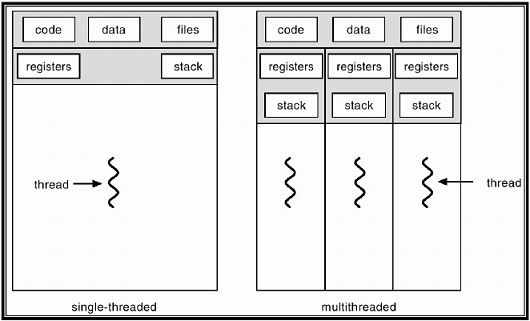
\includegraphics{threading.png}
    \end{center}

    \ \\
    \textbf{Advantages of Threads}
    
    \ \\
    The list below provides some of the most popular incentives for utilizing multithreaded programming.  For further reading, there is a variety of readily available literature pertaining to the topic (The author recommends \textit{Programming with POSIX Threads} by Butenhof).  
    
    \begin{itemize}
        \setlength\itemsep{-0.1em}
        
        \item \emph{Faster Execution}: Threads can take advantage of computer systems which possess multiple CPUs.  Instead of being bound to doing one sequence of instructions at a time, the only limitation is the number of processors available.  This scales from small personal computers to massive supercomputers.  
        \item \emph{Lower Resource Consumption}: Threads spare the kernel from having to do significant amounts of computation.  By sharing the parent's address space, less time is required in kernel mode doing work not pertinent to the problem.  Additionally, by utilizing the same address spaces, less memory management must be performed during switching.  
        \item \emph{Better System Utilization}: Most code is inherently parallelizable even though it is traditionally envisioned as sequential.  Any number of disjoint tasks can be executed in parallel instead of in a sequence.  A classic analogy for parallelization envisions a house with 5 rooms to be painted.  Assuming that painting a room is an individual task that cannot be subdivided, up to 5 painters can be hired to paint the house.  Painting some rooms may take longer than others, but overall, having 5 painters will always be much faster than just one.  
        \item \emph{Simplified Sharing \& Communication}: Since threads can share data structures (given that they have a common heap space), passage of information between threads is simple and does not require kernel intervention (as is usually required in traditional IPC mechanisms).  
        
    \end{itemize}

\end{myindentpar}

\ \\
{\large \underline{Assignment}:}

\begin{myindentpar}{5mm}

	You are given 5 files: client\_E7.cpp, dataserver.cpp, request\_channel.cpp, request\_channel.h, and a functional makefile. When you type the command 'make' into your shell prompt, two executables will be produced: client and dataserver.  
	
	\ \\
	The code given to you is functional.  You may type ./client (With no arguments) to observe execution and behavior of the system. The client process calls fork() and runs the dataserver program.  Afterwards, it populates a request buffer with 300 requests, 100 each for three hypothetical users: John Smith, Jane Smith, and Joe Smith. This is done using one, single-threaded process.  The preprogrammed argument, -n, allows you to specify the number of requests \emph{per person}.  For example, typing "./client -��n 10000" would cause 30000 requests to be generated (10000 per person).  Since the program is single threaded, you should observe that the program will run much slower with 100 times more work to do.  
	
	\ \\
	In large systems, it is quite possible that the number of requests could grow exponentially.  Websites like Amazon receive around 80 million requests daily.  Other companies such as Google and Youtube, receive requests numbering in the hundreds of millions.  No single process will ever be able to this volume of traffic.  So, how do the worlds largest businesses handle it in stride?  Instead of making one process do all of the work, multiple processes handle data requests concurrently.  In doing so, it is possible to handle large quantities of data since one can continue to add more cores/process threads to the system as load increases.  
	
	\ \\
	In this assignment, you are to increase the efficiency of the client-server program given to you by using multithreading.  You must add a command line option, -w, which allows users to enter a number.  This number will define how many worker threads your program will utilize.  Your program must spawn that many worker threads successfully, and these threads must work together to handle all of the requests provided to it.
	
	\ \\
	Multithreading often requires the use of specialized "thread-safe" data structures. In order to facilitate multithreading, you will code a thread-safe class called SafeBuffer (see the commented-out line client\_E7.cpp, "//SafeBuffer request\_buffer;"). SafeBuffer can simply wrap around an STL data structure (we recommend std::list or std::queue), but must have a constructor and destructor as well as the operations push\_back and retrieve\_front (if you want the provided make\_histogram function to work, also include a size function). push\_back adds an element to the back of the buffer and retrieve\_front removes an element from the front so that items are added and removed in FIFO order (see requirements below). Both functions must use locks (see Advanced Concepts section) to ensure that the buffer can be modified concurrently at either end (concurrent modification at \emph{both} ends requires \emph{semaphores}, which we will tackle in the next assignment).
	
	\ \\
	In addition to processing the requests using multithreading, and coding a specialized data structure for that purpose, the request buffer must also be initially populated using multithreading. However, writing the code for request threads will be much easier than the worker threads: you will only ever have 3 request threads, one for each user (John, Jane, and Joe from earlier; note we said 3 request \emph{threads}, not 3 request \emph{thread functions}), and each one simply pushes n requests (corresponding to its respective user) to request\_buffer. Furthermore, the request threads do not have to run concurrently with the worker threads (and in fact \emph{must} not), which means that the only lines of request-thread-related code in main (apart from setting up the thread parameters) will be three pthread\_create calls followed by thread pthread\_join function calls.
	
	\ \\
	Aside from multithreading, your program should have the following characteristics and satisfy the following requirements:
	\begin{itemize}
	    \setlength\itemsep{-0.1em}
	    
	    \item The program should function correctly for any number of threads. This does not mean that you have to handle all the errors resulting from large numbers of threads, but only that high numbers of threads do not in and of themselves affect program correctness. Practically speaking this means that your synchronization is provably correct, not that your error-handling is robust. You will not have to test your program with more threads than the minimum of (fd-max - 2)/2, and however many threads causes pthread\_create to fail. The value of fd-max on your system can be checked with "ulimit -n" at the command line, while the number of threads that causes pthread\_create to fail may need to be determined experimentally. Note that both values differ greatly between operating systems.
	    \item No fifo files should remain after running the client program with any number of threads.  
	    \item The client program should not take an unreasonably long time to execute.  Generally, the execution should be quicker than the single threaded version.  You can use the sample code as a performance baseline.  
	    \item All requests for the program are handled correctly, which includes being processed in FIFO order.  The histogram should report the correct number of requests and should NOT drop any requests.  
	    \item Your code may not make use of \emph{any} global variables, as they (in most circumstances) exemplify poor programming practice. The easiest way to avoid this is by using storage structs (more on those later).
	    
	\end{itemize}

	\ \\
    \textbf{Bonus}
    
    \ \\
    You have the opportunity to gain bonus credit for this machine problem. To gain this bonus credit, you must implement a real-time histogram display for the requests being processed.
    
    \ \\
    Run the initial client code once, and pay close attention to the final display. It uses the make\_histogram\_table function to format and output the frequency counts for the requests processed for each patient, which takes as arguments the 3 patient names and pointers to the 3 *frequency\_count vectors (ctrl+F in the initial code can help you figure out what the frequency\_count vectors are).
    
    \ \\
    Write a signal-handler function that clears the terminal window (system("clear) is an easy way to do this) and then displays the output of make\_histogram\_table. You will need to make sure that this is threadsafe by synchronizing on the same mutexes that the worker threads use to modify the *frequency\_count vectors.
    
    \ \\
    In main, register your signal-handler function as the handler for SIGALRM (man 2 sigaction). Then, set up a timer to raise SIGALRM at 2-second intervals (man 2 timer\_create, man 2 timer\_settime), so that your handler is invoked and displays the current patient response totals and frequency counts approximately every 2 seconds. To do this, you will need to make sure that your signal handler is given all the necessary parameters when it catches a signal (man 7 sigevent). When all requests have been processed, stop the timer (man 2 timer\_delete).
    
    \ \\
    If you have succeeded, the result should look like a histogram table that stays in one place in the terminal while its component values are updated to reflect the execution of the underlying program. 
    
    \ \\
    Is there some purpose for this bonus portion other than making your program output look nice? Yes, there is. Firstly, it gives you the opportunity to use signals and signal handlers (perhaps for the first time), which are important both in this course and generally in computer science. Secondly, it provides a snapshot of the run-time state of your program, which can be useful for debugging (i.e. if you can tell that the histogram is updating but the values aren't changing, you know there's a problem to be diagnosed).
    
    \ \\
    As with the other parts of the assignment you will lose points for using global variables. However, using global variables for the bonus will result in points being deducted \emph{only from the bonus portion of the assignment}, not from the main assignment, i.e. you cannot lose points by attempting to earn the bonus credit. Finally, please use the make\_histogram\_table function to format your output. Programming assignments are much easier to grade when the output is standardized.

\end{myindentpar}

\ \\
{\large \underline{Deliverables}:}

\begin{itemize}
    \setlength\itemsep{-0.1em}

    \item \textbf{Code:}
    \begin{itemize}
        \setlength\itemsep{-0.1em}
        
        \item You are to turn in one file ZIP file which contains the files provided in the sample code, modified to fulfil the requirements of the assignment.  Along with this, turn in the report (described below) and any other code that your program requires to run.  
        \item If your program requires specific steps to compile and run, please provide a README file that describes these steps.  (Please do try to keep it to only a makefile.  You shouldn't need to do anything fancy or convoluted)
        
    \end{itemize}

    \item \textbf{Report:}
    \begin{itemize}
        \setlength\itemsep{-0.1em}
        
        \item Once you've finished all programming tasks, author a report that answers the following questions about your code:
        \begin{enumerate}
        
            \item Describe what your code does and how it differs from the code that was initially given to you.  
            \item Make a graph that shows how your client program's running time for n = 10000 varies with the value for "w".  Include at least 20 datapoints (more or less evenly spaced) starting at 5 and going to the highest number that will run (\emph{without} reporting some kind of error) on your OS.  After making the graph, describe the behavior of the client program as w increases.  Is there a point at which the overhead of managing threads in the kernel outweighs the benefits of multithreading?  Also compare (quantitatively and qualitatively) your client program's performance to the code you were originally given.
            \begin{itemize}
                \setlength\itemsep{-0.1em}
                
                \item Note: Timing may be done in several ways.  One way is to use the time command from the shell (See the time manual page using the command man 1 time).  Another would be to time your program internally using either clock\_gettime() or gettimeofday() (see corresponding manpages man clock\_gettime and man gettimeofday). 
                
            \end{itemize}
            
            \item Describe the platform that you gathered data on (I.e. CSCE Linux server, Raspberry Pi, personal computer, etc...).  If it was a personal device (this includes the raspberry pi), describe the operating system that it runs.  Also answer the following sub-questions:
            \begin{itemize}
                \setlength\itemsep{-0.1em}
                
                \item What is the maximum number of threads that the host machine will allow your client program to create before reporting an error? What error is reported?
                \item What does the operating system do when your client program tries to create more threads than allowed?
                \item How does your client program behave in response?
                
            \end{itemize}
            
        \end{enumerate}
        
    \end{itemize}
    
\end{itemize}

\noindent
\ \\
{\large \underline{Notes Concerning Global Variables and Storage Structs}}

	\ \\
	Global variables are generally regarded as poor coding practice, but we realize that some students haven't yet been taught how to avoid using them in a multithreaded program, where they seem to be a very easy and attractive option. Here, then, is the way we have found easiest and most effective to avoid using global variables: storage structs.
	
	\ \\
	A storage struct is an old-fashioned C struct, which serves mainly to store and organize different variables. An instance of such a struct can be  passed to a thread function as the last argument given to pthread\_create. The thread function then accesses its arg parameters, a void pointer, and casts it back to the type of the storage struct that is being used, and is then able access all the struct's fields and methods. If a programmer cleverly defines the struct's fields based on the needs of his program, he has a very clean and efficient way to pass parameters to a thread function.
	
	\ \\
	Instances of storage structs can be declared and initialized in main, and any memory allocated for them is valid so long as it remains in scope in main. This means that pointers to storage structs that have been allocated in main, and to their data fields, can be passed to thread functions and will be valid until main terminates. Even then, if heap memory is used it will be valid until explicitly deleted. Pointers and storage structs can thus be used to solve the scoping problems previously solved by global variables, making the latter unnecessary.

	\ \\
	You may find it helpful to go over the example code in the man page for pthread\_create, since it includes an example of storage struct usage (the thread\_info struct).

\newpage
\noindent
\ \\
{\large \underline{Notes Concerning the Graph for your Report}}
\ \\
\begin{tikzpicture}
\begin{axis}[
	title=MP7 Timing Data,
	xlabel=Number of Worker Threads ({$w$}),
	ylabel=Execution Time (in {$\mu$}-secs),
]
\addplot table [x=w, y=usecs, col sep=comma] {testdata.csv};
\end{axis}
\end{tikzpicture}

        \ \\
        This graph was created using data gathered on a MacBook Pro 2011 running OS X Sierra, with n held constant at 10000. You will not be expected to gather this many data points (there are more than 60 in this graph), or run 1900 threads, for your report. Gathering this much data required increasing the number of available file descriptors as root, as well as more error-handling code that you will be expected to write.
        
        \ \\
        It does, however, demonstrate the expected behavior of MP7 as w increases, and is intended to encourage you to test your program with larger numbers of threads than you might initially be inclined to. After all, the report requires you to test right up to the default limitations of your OS (but no further).
        
        \ \\
        If, in gathering data for your report, you find that the default limitations of your OS (namely, available file descriptors and thread creation resources) prevent you from building a graph that demonstrates the full range of MP7's expected behavior (i.e. performance increases, then flattens out, then suddenly becomes horrible), not to worry: you are only required to run as many threads as your OS will allow \emph{by default}. But you will not be able to complete Part 3 of the report if you try to do less.


\ \\
{\large \underline{Advanced Concepts}:}

\begin{myindentpar}{5mm}

    \noindent
    \textbf{Atomic Operations \& Race Conditions}
    
    \ \\
    The scheduler (process 0 on UNIX/Linux machines) makes all decisions regarding when processes execute and in what order.  The choice of which process to execute next is made by complex algorithms which strive for efficiency and fairness (all processes get a chance).  However, the order of execution is not defined by these algorithms (i.e. there is no enforced execution sequence given a list of processes to be run).  As a result, processes are switched in and out of execution depending on the will of the system's scheduling algorithm.  

    \ \\
    UNIX processes are known as preemptive or reentrant (both terms mean the same thing).  Reentrant processes are those which can be context switched in the middle of execution and then resumed later.  This means that operations such as function calls, file I/O, and even system calls can and will be interrupted during execution and resumed later.  
    
    \ \\
    There are some operations that are so fundamental to the system and the hardware that they cannot be interrupted.  They either run to completion or not at all.  These are known as atomic operations.  Most instructions that can be implemented as a single assembly language instruction are atomic.  These assembly language statements are executed directly on the processor in one clock cycle.  Add with two arguments, subtract with two arguments, load a word from memory, store a word to memory, etc. are all atomic operations.  Anything more complex, such as adding three+ arguments, can be divided into more than one assembly instruction.  As a result, they are not atomic and can potentially be interrupted.  
    
    \ \\
    In the context of normal processes, interruptions are fine.  As long as the state is resumed properly, the user is never aware that their program was interrupted (potentially several times).  When a program uses threads, however, the results can be disastrous.  As a thought experiment, imagine a process containing two threads (1 \& 2) and a set of shared global variables.  If both threads attempt to execute code to modify any of these variables, the result is dependent on the order in which the two threads execute.  The order of thread execution is impossible to predict.  By default, there are no guarantees, and every possible situation can and could happen.  Situations like this, where the result is dependent on the order of execution, are known as \emph{race conditions}.  The figure below illustrates the above situation and shows all possible interleavings of code execution for a given set of instructions.  
    
    \begin{center}
        Figure \textbf{XXX}: Race Condition
    \end{center}
    \begin{center}
        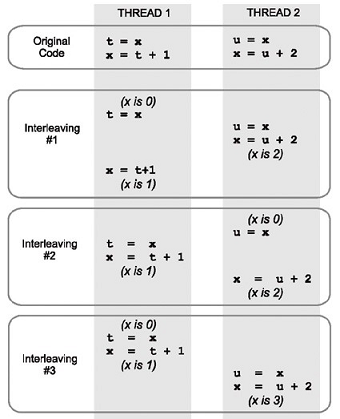
\includegraphics{race_condition.png}
    \end{center}

    \ \\
    \textbf{Synchronization}
    
    \ \\
    A segment of code that potentially could be damaging if caught in a race condition is known as a critical section.  Critical sections must be executed atomically with respect to all other threads in the system.  Even though system calls and functions generally aren't atomic, they can be made atomic through the use of synchronization.  This means that when a process calls an function or performs an operation, the function or operation will complete fully or not at all without another process or thread performing the same operation.  There are multiple ways of making complex expressions into atomic operations, such as locks and semaphores.  Many of these methods will be covered in extensive detail in lecture.  Consequently, this section focuses on the synchronization method that you should use for this assignment: the pthread mutex.  
    
    \ \\
    A mutex, short for "mutual exclusion," prevents two concurrently running threads from entering the same section of code at the same time.  The POSIX API that you'll be using in this maching problem provides some very convenient functions for using mutexes.  To use them, be sure to add "\#include$<$pthread.h$>$" to your program.  Mutex types can be declared like any other variables (i.e. pthread\_mutex\_t temp;) and passed by address to the relevant API calls, such as pthread\_mutex\_init(\&temp, NULL).  
    
    \ \\
    A list of relavant API calls along with short descriptions of each is provided below:
    \begin{enumerate}
        \setlength\itemsep{-0.1em}

        \item \textbf{pthread\_mutex\_lock(pthread\_mutex\_t *mutex)}
        
        \ \\
        When a process calls lock on a mutex, one of two things will occur.  If no other process has the mutex locked, the mutex becomes locked, and the process continues on into the critical section that follows.  If another process has control over the mutex (i.e. it is locked by another process), the process that just called for the lock is put to sleep.  Any other processes that call lock while the mutex is locked will also be put to sleep.  
        
        \ \\
        All threads must utilize the same pthread\_mutex\_t object or they will not be synchronized.  
        
        \ \\
        For more information about the use of this function, consult the manual page using the shell command \code{man 3 pthread\_mutex\_lock}.  
        
        \ \\
        Important note about POSIX thread manpages: Your Linux/UNIX machine (such as a raspberry pi) may not come with certain manpages by default.  In order to acquire them, you will need to instal lthe package \code{manpages-posix-dev} using the installation mechanism required by your distribution.  For the raspberry pi running raspbian, the command is: \code{sudo apt-get install manpages-posix-dev}.  
        
        \vspace{-7mm}
        \ \\
        \item \textbf{pthread\_mutex\_unlock(pthread\_mutex\_t *mutex)}
        
        \ \\
        Calling this function releases (unlocks) a mutex that had previously been locked by pthread\_mutex\_lock.  If there is another process waiting to lock the mutex, that process is woken up and given the lock.  Afterwards, the whole process starts over again.  For more information, consult \code{man 3 pthread\_mutex\_unlock}.  
        
        \vspace{-7mm}
        \ \\
        \item \textbf{pthread\_mutex\_init(pthread\_mutex\_t *mutex, const pthread\_mutexattr\_t *attr)}
        
        \ \\
        This function initializes the mutex referenced by \emph{mutex} to the attributes specified by \emph{attr}.  (Note: In this machine problem, attr can always be NULL and \emph{mutex} will automatically be initialized using default values).  It returns 0 if mutex initialization was successful or an error value if it failed.  For more information, consult \code{man 3 pthread\_mutex\_init}.  

        \vspace{-7mm}
        \ \\        
        \item \textbf{pthread\_mutex\_destroy(pthread\_mutex\_t *mutex)}
        
        \ \\
        Uninitializes the mutex passed as an argument.  As always, for more information, consult \code{man 3 pthread\_mutex\_destroy}.  
        
    \end{enumerate}

\end{myindentpar}

\newpage
\noindent
{\large \underline{Rubric}:}

\begin{itemize}
        \setlength\itemsep{-0.1em}
        
        \item Request Threads (20 points)
        		\begin{enumerate}
        		\setlength\itemsep{-0.1em}
        			\item Initial code modified to create 3 request threads in main. (15 points, all or nothing)
			\item Coded one, \emph{and only one}, request\_thread\_function, and not 3 separate copies of it (one for each user). If 3 such copies are used, deduct 10 points. The person's name must be passed as an argument, or as one of the member variables an appropriate storage struct.
			\item Request threads joined before any worker threads are started. (5 points)
		\end{enumerate}
	\item Worker Thread Functionality (30 points)
		\begin{enumerate}
		\setlength\itemsep{-0.1em}
			\item Quits properly using "quit" request pushed from main function. (10 points)
			\item Histograms correct (must use make\_histogram\_table function). (10 points)
			\item Proper thread-safety used for request\_buffer and *frequency\_count vectors. (10 points
				\begin{itemize}
				\setlength\itemsep{-0.1em}
					\item SafeBuffer used for request\_buffer.
					\item Locks used before incrementing *frequency\_count vectors.
				\end{itemize}
		\end{enumerate}
	\item Globals (or rather, lack thereof) (10 points)
		\begin{enumerate}
        		\setlength\itemsep{-0.1em}
			\item No global variables used, if global variables are used deduct from 1 to 10 points depending on how many.
			\item No points deducted for global variables that are used \emph{only for the bonus portion of the assignment}.
		\end{enumerate}
	\item Cleaning up resources (20 points)
		\begin{enumerate}
		\setlength\itemsep{-0.1em}
			\item All dynamically-allocated objects cleaned up. (i.e. no memory leaks) (10 points)
			\item All fifo special files removed via "quit" and proper destructor usage (even in case of errors) (10 points)
				\begin{itemize}
				\setlength\itemsep{-0.1em}
					\item fifo special files (man 7 fifo) will be present during program execution while they are being used, but all 10 points will be lost \emph{if any fifo files remain after program termination}.
				\end{itemize}
		\end{enumerate}
	\item Report (20 points)
		\begin{enumerate}
        		\setlength\itemsep{-0.1em}
			\item Results demonstrated using plots/graphs (5 points)
			\item Run-time variation observed in the plots (9 points)
				\begin{itemize}
        				\setlength\itemsep{-0.1em}
					\item Plot should be linear with w for some range, but should begin flatten out (or even decrease!) after a certain point when thread/channel management starts to outweigh the benefits of parallelization.
				\end{itemize}
			\item Answers provided to the 3 questions in the Report section of the handout (6 points, 2 for each question)
		\end{enumerate}
	\item Bonus Real-time Histogram Display (value to be determined by professor)
		\begin{enumerate}
			\item No global variables used for this portion of the assignment.
			\item Uses the provided make\_histogram\_table function.
			\item Looks good and works.
		\end{enumerate}
\end{itemize}

\newpage
\noindent
{\large \underline{Bibliography}:}

\ \\
{[} 1 {]} \hspace{1.2mm} Northwood, Chris. "Computer Science Notes $\Rightarrow$ Operating Systems." Operating
\hspace*{1.15cm} Systems. N.p., n.d. Web. 03 June 2016.

\ \\
{[} 2 {]} \hspace{1.7mm} Iwillgetthatjobatgoogle. "Race Conditions: First Approach." I Will Get That Job
\hspace*{1.05cm} At Google. N.p., n.d. Web. 03 June 2016.


\end{document}

